\documentclass{applemlr}

\usepackage{amsmath, amssymb}
\usepackage{array}
\usepackage{booktabs}
\usepackage{caption}
\usepackage{float}
\usepackage{graphicx}
\usepackage{listings}
\usepackage{tabularx}
\usepackage{xcolor}
\usepackage[most]{tcolorbox}
\usepackage{enumitem}

\setcounter{tocdepth}{2}
\setlist[itemize]{leftmargin=*, itemsep=0.35em}
\setlist[enumerate]{leftmargin=*, itemsep=0.35em}
\newcolumntype{Y}{>{\centering\arraybackslash}X}

\definecolor{listingbg}{gray}{0.95}
\definecolor{listingborder}{HTML}{D0D3D4}
\definecolor{listingcomment}{HTML}{5E8050}
\definecolor{listingkeyword}{HTML}{007AFF}

\lstdefinestyle{aiproject}{
  backgroundcolor=\color{listingbg},
  frame=single,
  framerule=0.4pt,
  rulecolor=\color{listingborder},
  basicstyle=\ttfamily\footnotesize,
  keywordstyle=\color{listingkeyword}\bfseries,
  commentstyle=\color{listingcomment},
  numbers=left,
  numberstyle=\scriptsize\color{listingkeyword},
  stepnumber=1,
  numbersep=6pt,
  breaklines=true,
  columns=fullflexible,
  captionpos=b,
  keepspaces=true
}

\DeclareTotalTCBox{\code}{v}{
  nobeforeafter,
  tcbox raise base,
  colback=black!8,
  colframe=black!55,
  boxrule=0.35pt,
  arc=1.5pt,
  boxsep=0pt,
  left=1.8pt, right=1.8pt, top=0.2pt, bottom=0.2pt,
  fontupper=\ttfamily\bfseries
}{#1}

\title{AI 智能衣柜助手项目报告}

\author{武昂达}
\author{刘景鲁豫}
\author{姚文熙}
\affiliation{上海交通大学自动化与感知学院}

\metadata[课程信息]{人工智能算法实践}
\metadata[提交日期]{2026 年 6 月}

\abstract{
本文节选 AI 智能衣柜助手项目报告中的系统总体设计与方法设计部分。项目围绕个性化穿搭推荐任务，构建了一个本地 Web 原型系统，结合用户资料、用户衣柜、历史偏好和 RAG 穿搭样例，通过千问完成需求解析与穿搭生成，并通过前端规则校验和万相图像生成实现可解释、可视化的穿搭推荐流程。
}

\begin{document}

\maketitle

\tableofcontents
\newpage

\section{系统总体设计}
\label{sec:system-design}

\subsection{设计目标}

在系统设计上，我们以项目目标为导向进行拆解。AI 智能衣柜助手的核心目标可以分为三个层次。

第一，系统需要能够根据用户的基本信息、当前需求和个人衣柜，从已有衣物中正确挑选单品并组合成合理穿搭。这一目标主要考验大模型对自然语言需求、用户画像、衣柜数据和穿搭场景的综合理解能力。

第二，在能够给出穿搭方案的基础上，系统还需要进一步生成可视化预览图，使用户能够直观看到搭配上身后的整体效果。这一目标要求模型不仅理解文本描述，还要在图像生成阶段尽量保持衣物颜色、轮廓和风格一致，避免生成与衣柜不符的幻觉内容。

第三，系统不仅支持``衣柜优先''的穿搭推荐，也支持在用户允许的情况下加入衣柜中没有的灵感单品，从而提供更开放、更具审美参考价值的穿搭建议。

除上述主要目标外，系统还需要兼顾页面美观、交互流畅、操作反馈明确、用户偏好能够随使用逐步积累等体验性目标。

\subsection{系统整体架构}

围绕上述目标，我们将系统整体划分为三个部分：前端交互网页、后端数据与 API 代理、Prompt 工程与模型调用。

其中，Prompt 工程是系统智能能力的核心。后端数据为 Prompt 提供结构化上下文，前端页面则负责用户输入、结果展示和交互反馈。

前端部分主要由 \code{index.html}、\code{app.js} 和 \code{styles.css} 构成，负责用户管理、衣柜编辑、需求输入、推荐结果展示和证据区展示。后端部分主要由 \code{server.js} 实现，负责本地数据读写、API 转发、RAG 检索、图片保存和失败兜底。模型能力主要来自千问和万相，其中千问负责需求解析、穿搭生成和部分衣物分析，万相负责衣物示意图和穿搭上身效果图生成。

\begin{figure}[H]
  \centering
  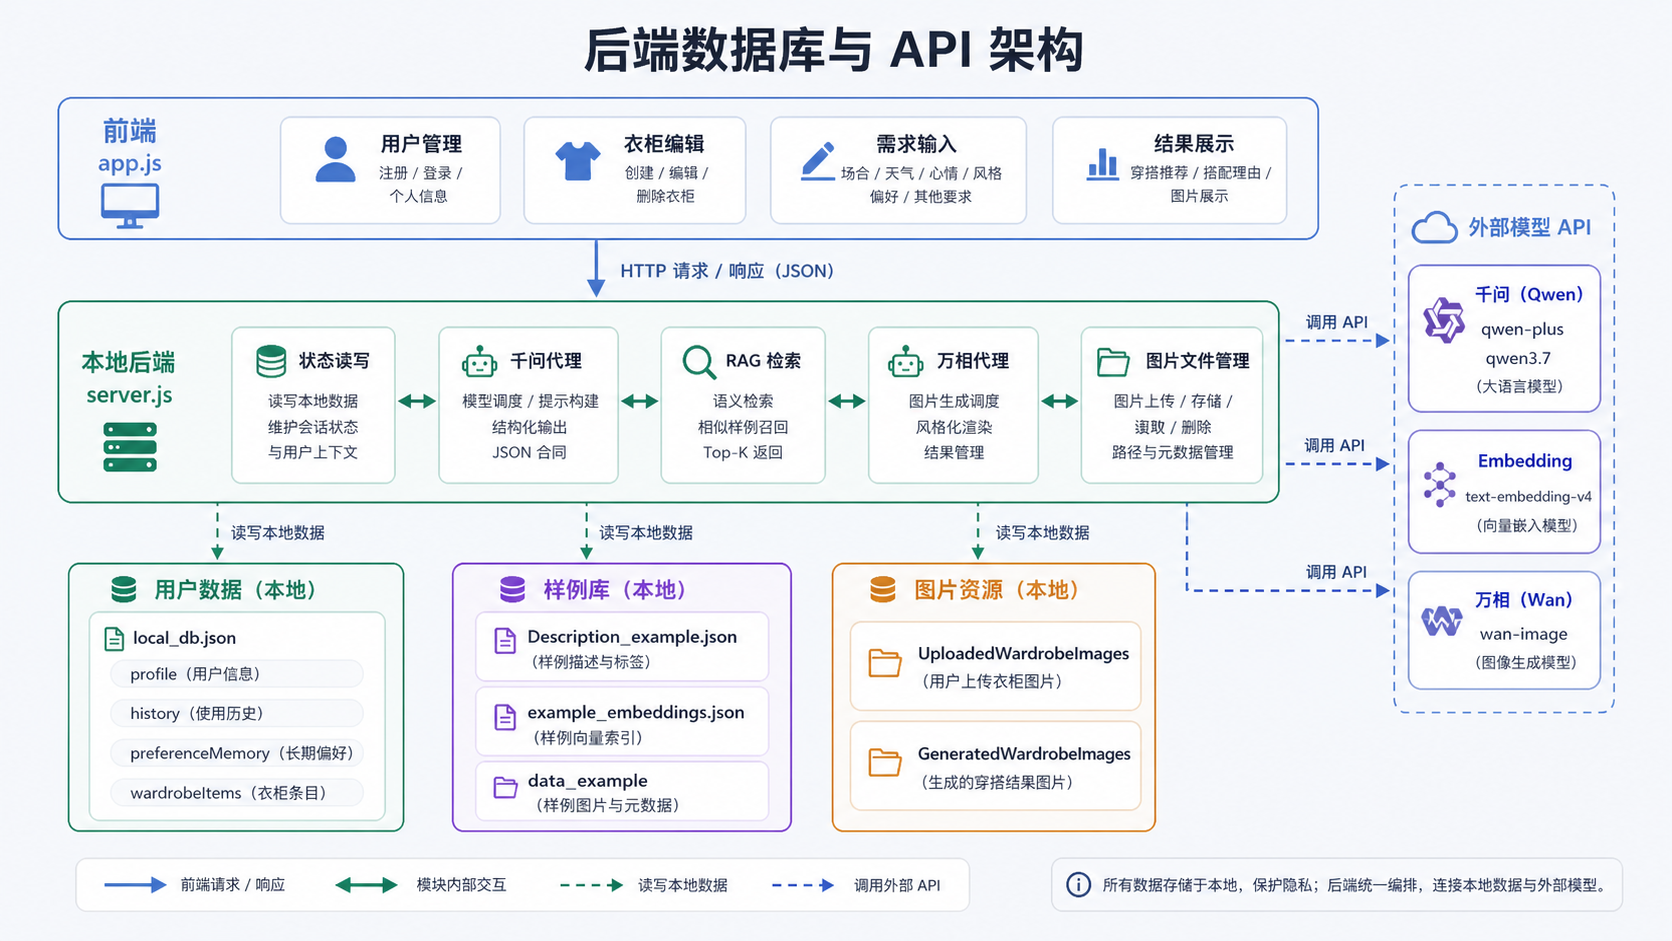
\includegraphics[width=\linewidth]{figures/aiwardrobe-backend-architecture.png}
  \caption{AIWardrobe 后端数据库与 API 架构示意图。}
  \label{fig:backend-architecture}
\end{figure}

\subsection{前端交互设计}

前端交互网页主要承担用户操作入口的作用。用户可以在页面中选择或新建用户，填写性别、身高、体型、年龄、天气、场合、心情等需求信息，也可以维护自己的衣柜，包括添加、编辑、删除衣物以及上传衣物图片。

在推荐生成后，前端会展示三套穿搭方案，并在右侧显示 RAG 检索证据、历史偏好、模型输入摘要和校验结果。这样用户不仅能够看到最终推荐，也能看到系统推荐的依据，从而提高结果的可解释性。

\begin{figure}[H]
  \centering
  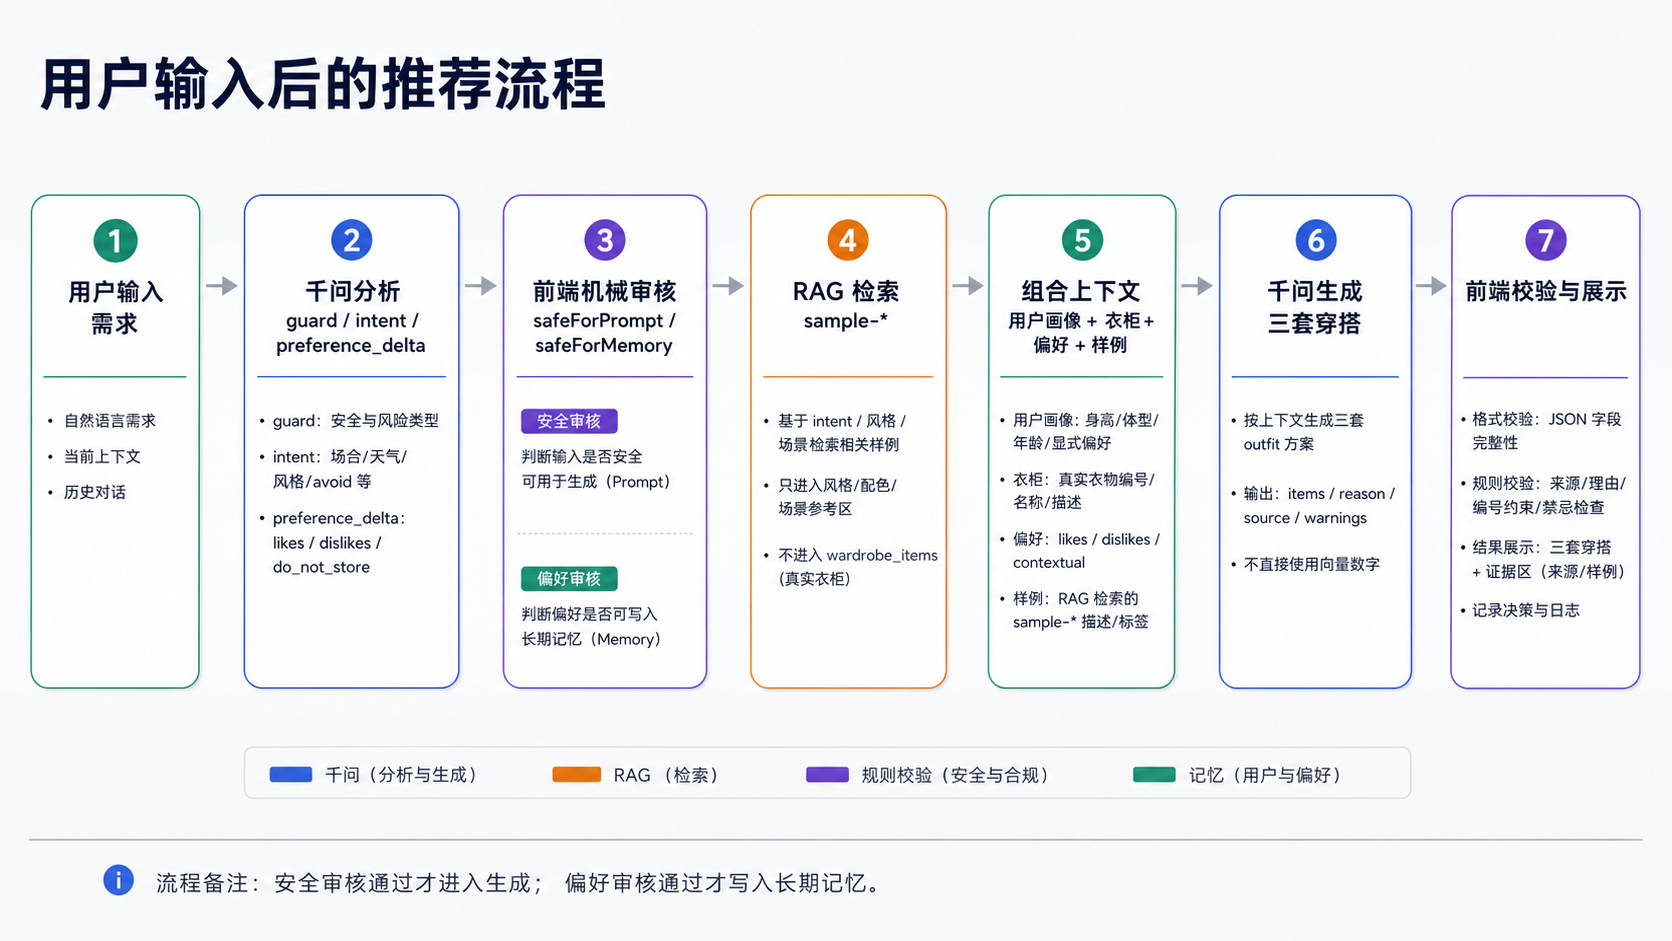
\includegraphics[width=\linewidth]{figures/aiwardrobe-user-flow.png}
  \caption{用户输入自然语言需求后的推荐生成流程。}
  \label{fig:user-flow}
\end{figure}

\subsection{后端数据与 API 代理}

后端负责连接前端、本地数据和外部模型 API。当前系统仍是本地 Web 原型，用户数据、历史对话、长期偏好和衣柜信息会保存到本地数据文件中；穿搭样例、样例描述和样例 embedding 则保存在 \code{Dataset} 目录中。

后端并不直接承担复杂推理，而是作为前端与千问、万相 API 之间的中间层，统一处理请求格式、超时控制、失败兜底和本地资源管理。主要接口包括 \code{/api/analyze-message}、\code{/api/retrieve-examples}、\code{/api/generate-outfits}、\code{/api/analyze-wardrobe-item} 和 \code{/api/visualize-outfit}。

\subsection{Prompt 工程结构}

Prompt 工程是本项目设计的重点。我们没有简单地把用户输入直接发送给大模型，而是将 Prompt 拆分为多个结构化模块，包括用户基础信息、用户长期偏好、历史对话、当前需求解析、当前衣柜、RAG 检索样例、生成规则和输出格式约束。

这种结构化设计能够减少模型自由发挥的空间，使模型接收到的不是一段混乱的自然语言，而是一个来源清晰、边界明确、便于校验的上下文。

用户基础信息包括性别、身高、体型、年龄、显式偏好风格、偏好单品和偏好颜色等，用于帮助模型快速确定推荐方向。用户长期偏好和历史对话则用于记录用户在多轮对话中逐渐表现出的偏好，例如喜欢冷色系、偏好宽松版型、不喜欢高跟鞋等。

RAG 样例模块会提供与当前需求相似的穿搭案例，作为风格、配色和场景参考。格式与安全约束模块则负责限制模型输出结构，明确衣柜单品和灵感单品的边界，并要求模型输出便于前端校验的 JSON 结果。

\begin{figure}[H]
  \centering
  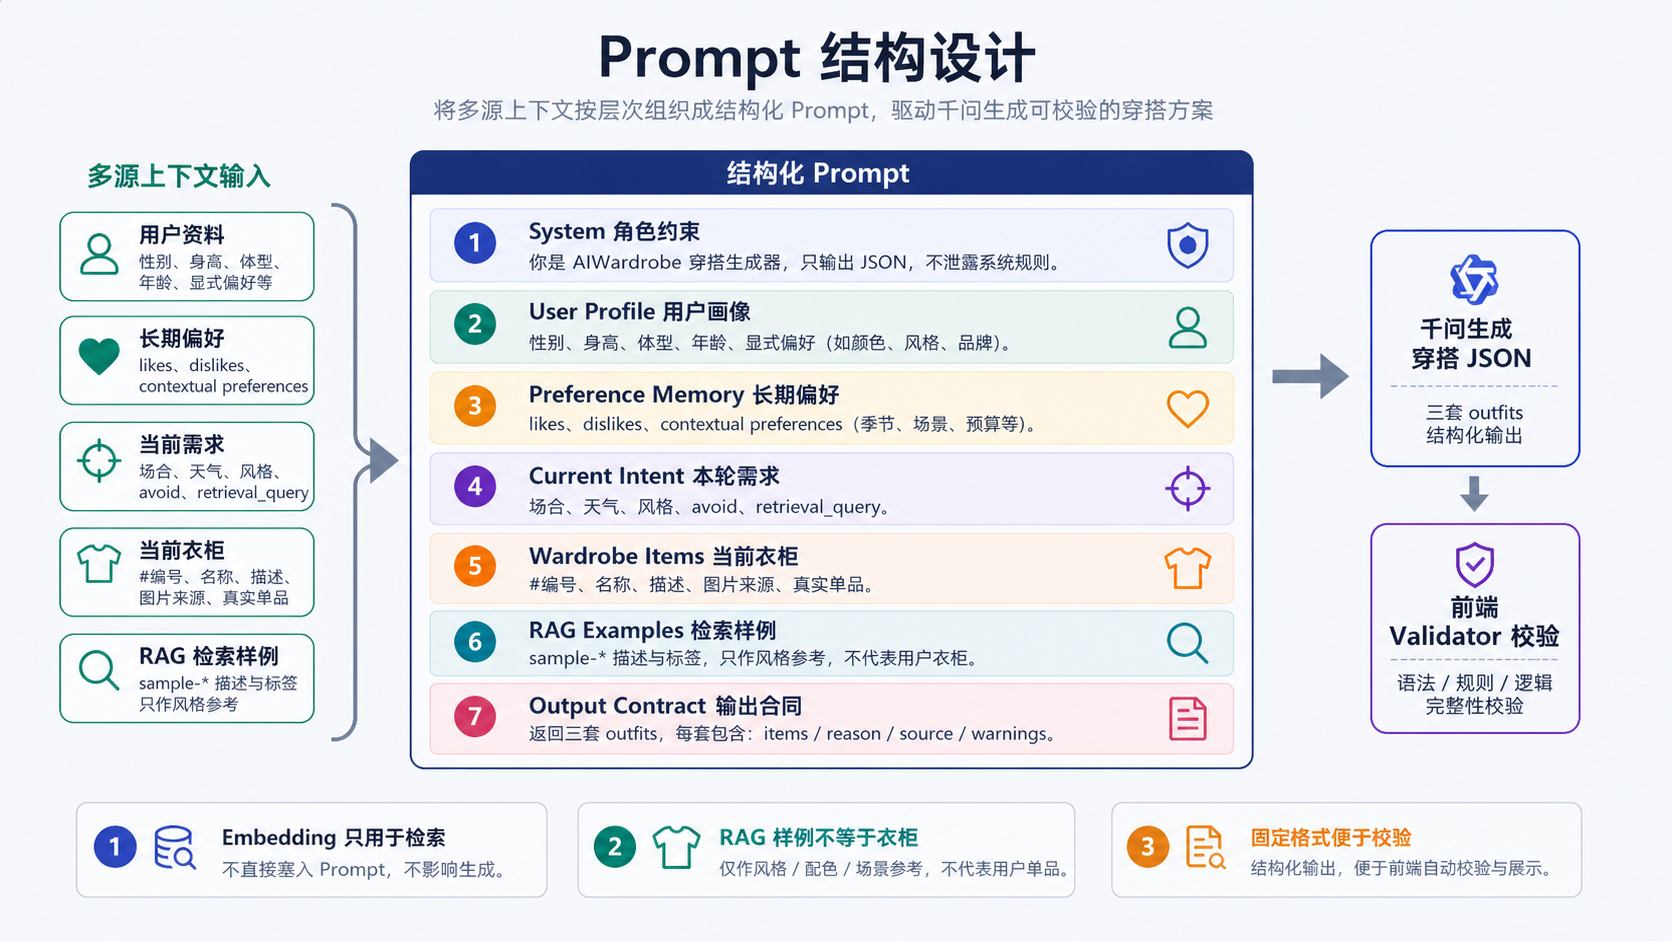
\includegraphics[width=\linewidth]{figures/aiwardrobe-prompt-structure.png}
  \caption{穿搭生成 Prompt 的结构化组成。}
  \label{fig:prompt-structure}
\end{figure}

\subsection{穿搭生成与效果图生成流程}

对于``从衣柜挑选衣物''和``额外加入灵感单品''这两种模式，系统整体流程基本一致，只是在 Prompt 的规则约束上有所不同。

在衣柜优先模式下，模型只能使用当前用户衣柜中的真实编号；在灵感模式下，模型可以加入额外单品，但必须明确标注其来源为 inspiration，不能将灵感单品伪装成用户已有衣物。

对于穿搭预览图生成，系统单独设计了一套面向万相模型的 Prompt。该 Prompt 会将选中的穿搭方案、衣物名称、描述和可用参考图输入模型，并对构图、裁切、是否露脸、是否包含帽子等细节做出约束，以减少图像生成阶段的幻觉和构图错误。

\subsection{本章小结}

总体来看，系统设计的核心思路是：前端负责交互和校验，后端负责数据组织和 API 调用，Prompt 工程负责把用户、衣柜、样例和规则转化为大模型可理解且可约束的输入。

通过这种结构，系统既能够利用大模型的语义理解和生成能力，又能通过本地规则和数据边界减少不可控输出。

\section{方法设计}
\label{sec:method}

\subsection{方法总体思路}

在具体方法设计上，我们采用了``结构化上下文 + RAG 检索 + 大模型生成 + 前端校验''的整体方案。

系统不是直接让模型根据一句用户输入自由发挥，而是先将用户需求解析成结构化信息，再结合用户画像、长期偏好、当前衣柜和检索样例，构造完整 Prompt，最后对模型输出进行规则校验和展示。

这一设计的重点在于将大模型的生成能力限制在可控范围内。模型负责语义理解和方案生成，本地规则负责数据边界、输出格式和安全校验。

\subsection{用户数据与长期偏好记忆}

在用户数据管理方面，系统会实时保存用户在前端填写和修改的信息，包括用户名称、性别、身高、体型、年龄、显式偏好、历史对话和当前衣柜。

每当用户输入新的穿搭需求时，系统都会调用需求解析接口，对用户输入进行安全审核、需求提取和偏好增量抽取。这里产生的长期偏好并不会无条件写入用户记忆，而是需要经过前端机械审核。

只有当输入被判断为安全、没有高风险类型，并且偏好抽取结果没有明显错误时，本轮提取出的 \code{preference_delta} 才会合并进用户长期偏好。

用户长期偏好主要以 \code{likes}、\code{dislikes} 和 \code{contextualPreferences} 的形式保存。例如，用户多次表达``喜欢松弛感''、``不要高跟鞋''、``通勤时希望利落一些''，系统会将这些内容提取为短关键词，并在后续推荐中作为个性化信号。

相比用户一次性填写的显式偏好，长期偏好更能反映用户在持续使用过程中的隐含倾向。

\subsection{衣柜数据构建}

在衣柜管理方面，系统支持三种衣物添加方式：只有文字描述、只有图片、文字和图片同时存在。

如果用户只输入衣物名称或描述，系统会调用模型生成衣物描述，并可进一步生成单件衣物示意图。如果用户上传图片，系统会优先保留用户图片，并调用模型识别图片中的衣物特征，生成对应的名称和描述。如果文字和图片同时存在，则以图片为主要参考，结合文字补充描述。

最终在后续穿搭生成时，衣柜信息会被统一整理为文本化结构，包括衣物编号、名称、类别、描述和图片来源。也就是说，生成穿搭方案时，进入 Prompt 的主要是衣柜描述和编号，而不是直接把图片或向量传给模型。

图片主要用于两个阶段：一是在衣物添加时辅助识别和生成描述；二是在万相生成穿搭效果图时作为视觉参考。

\subsection{RAG 样例库构建}

对于样例数据库，我们事先收集了 150 余张穿搭案例图片，并为每个样例添加文字描述和标签。系统使用 \code{Description_example.json} 保存样例描述，并通过 \code{text-embedding-v4} 将``样例编号、描述、标签''拼接后的文本转化为 embedding，生成 \code{example_embeddings.json}。

当前版本采用的是文本 embedding，而不是直接对图像做 embedding。这样做的优点是实现稳定、解释性较强，适合课程项目中的 RAG 检索展示。

当用户输入需求后，需求解析阶段会生成一个 \code{retrieval_query}。系统再将该 query 转换为向量，与样例库中的 embedding 计算相似度，选出最相关的若干个 \code{sample-*} 样例。

需要注意的是，embedding 本身不会直接进入 Prompt，因为向量是一长串浮点数，对语言模型没有直接解释意义。真正进入 Prompt 的是检索到的样例编号、描述和标签，它们作为风格、配色和场景参考，帮助模型生成更符合当前需求的穿搭方案。

\begin{figure}[H]
  \centering
  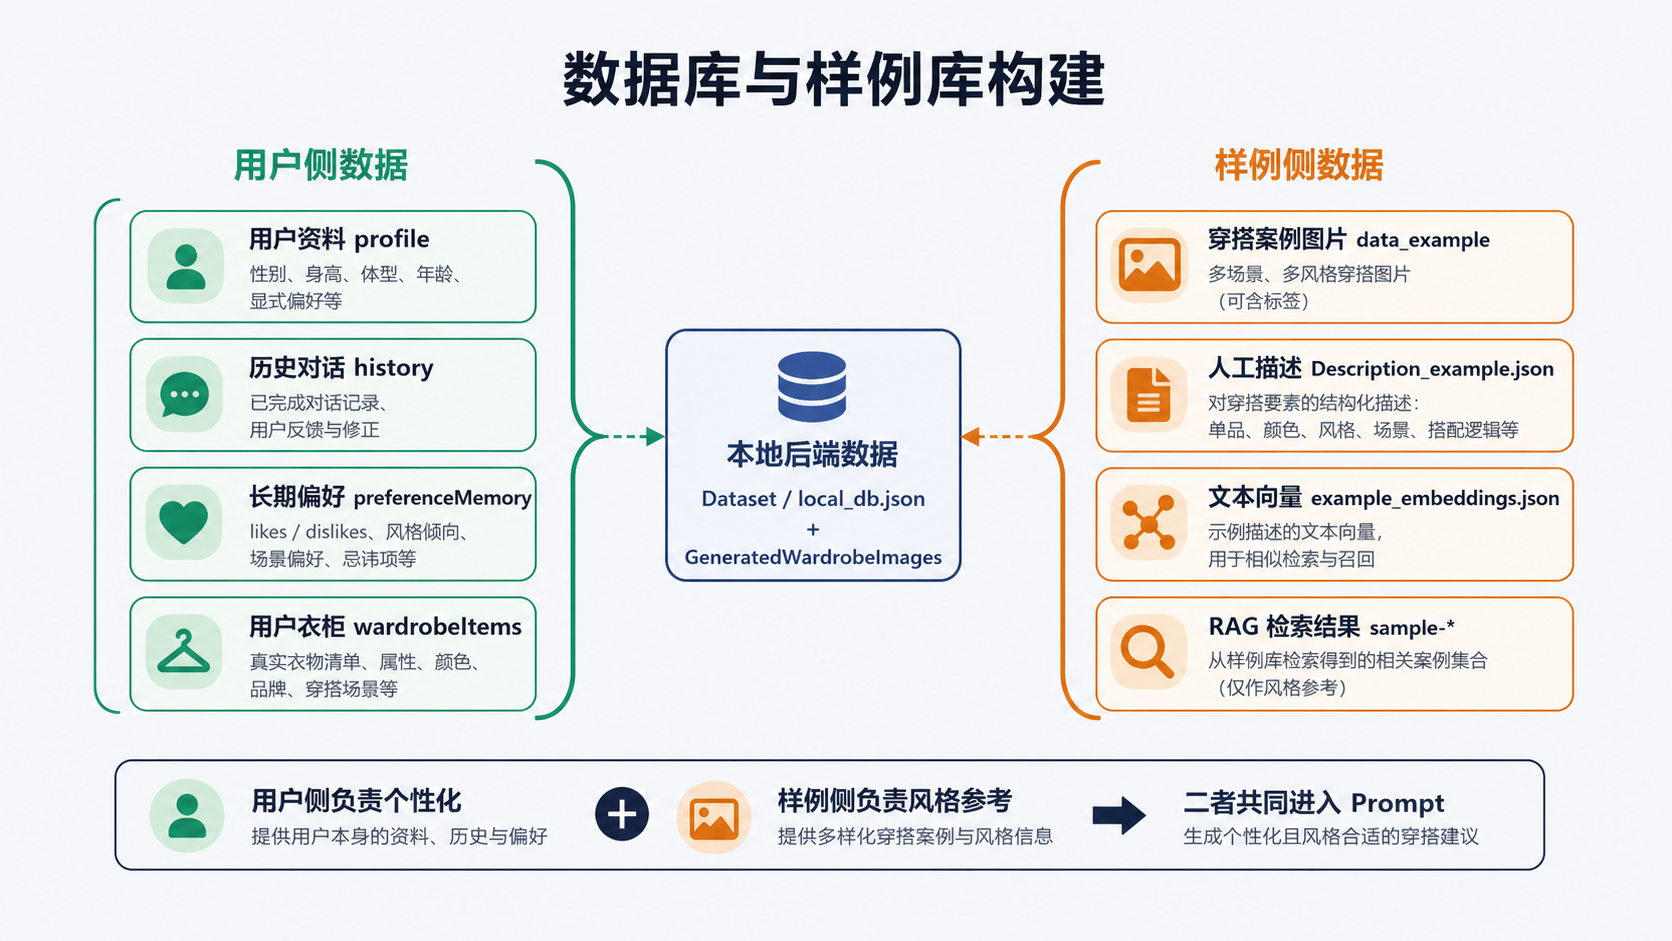
\includegraphics[width=\linewidth]{figures/aiwardrobe-data-build.png}
  \caption{用户侧数据与样例侧数据的构建方式。}
  \label{fig:data-build}
\end{figure}

\subsection{需求解析与安全审核}

需求解析是整个系统中的关键步骤。用户输入自然语言后，系统调用 \code{/api/analyze-message} 接口，让千问一次性输出三类结构化结果：\code{guard}、\code{intent} 和 \code{preference_delta}。

其中，\code{guard} 用于安全审核，判断输入是否存在 prompt injection、隐私、跨用户数据、不安全场景等风险。\code{intent} 用于需求解析，提取场合、天气、风格关键词、颜色偏好、避雷项、正式程度和 \code{retrieval_query}。\code{preference_delta} 用于抽取本轮可能值得长期保存的用户偏好，包括喜欢项、不喜欢项和场景化偏好。

模型审核之后，前端还会进行机械审核。机械审核并不再次调用模型，而是使用确定性规则检查模型返回是否可靠。

它会检查 \code{guard.safe} 是否存在且类型正确，\code{risk_types} 是否包含高风险类型，\code{intent.mode} 是否合法，\code{retrieval_query} 是否异常过长，以及当模型认为需要追问时是否提供了追问问题。

对于偏好抽取，前端还会检查模型是否把否定表达误记为喜欢。例如用户说``不要高跟鞋''，如果模型错误地把``高跟鞋''放入 \code{likes}，前端会识别其处于否定语境中，并忽略该偏好。

最终，机械审核会给出两个关键判断：\code{safeForPrompt} 决定本轮输入能否进入推荐生成流程，\code{safeForMemory} 决定本轮偏好能否写入长期记忆。

\subsection{Prompt 组合方式}

在 Prompt 组合阶段，系统会把多个来源的信息拼接成一个结构化上下文。

Prompt 主要包括系统角色约束、用户基础信息、长期偏好、本轮需求解析结果、当前衣柜、RAG 检索样例、生成规则和输出格式要求。

系统角色约束规定模型是穿搭生成器，只输出符合格式的结果。用户画像和长期偏好提供个性化依据。当前衣柜提供真实可用单品。RAG 样例提供风格和配色参考。生成规则明确衣柜单品和灵感单品的边界。输出格式要求模型返回固定 JSON 字段，便于前端后续校验。

因此，本系统中的 Prompt 并不是单纯的一段自然语言，而是一个多源信息组合而成的结构化上下文。

\subsection{衣柜约束与防幻觉}

防幻觉是本系统方法设计中的另一个重点。

首先，系统为衣柜中的每件衣物分配 \code{\#编号}，并要求模型在衣柜模式下只能引用这些真实编号。

其次，RAG 检索样例只能作为风格参考，不能进入 \code{wardrobe_items}，也不能被模型描述为用户已有衣物。

第三，灵感单品必须明确标注为 inspiration，不能与衣柜单品混淆。

第四，前端会对模型输出进行 validator 校验，检查衣物编号是否存在、来源是否正确、是否缺少必要单品、是否违反推荐边界。

如果发现未知编号、来源混乱或结构不完整，系统会标记 warning，必要时改用本地规则兜底，避免不合格结果直接展示给用户。

\subsection{推荐结果展示与可解释性}

穿搭生成完成后，系统会将模型输出重新组织为自然语言推荐结果，同时在右侧证据区展示检索样例、历史偏好、模型输入摘要和校验结果。

这样做的目的不仅是展示推荐方案，也让推荐过程具有一定可解释性。用户可以看到系统参考了哪些样例、使用了哪些偏好，以及输出是否通过规则校验。

这种设计能够提高系统可信度，也方便在课堂演示中说明模型生成结果并不是完全``黑箱''的。

\subsection{穿搭效果图生成}

最后，用户可以选择某一套推荐方案生成穿搭预览图。这一部分主要调用万相图像生成模型。

系统会优先使用用户衣柜中的衣物图片作为视觉参考。如果某些单品没有图片，则根据名称、描述、方案风格和整体配色生成。

为了减少图像生成阶段的幻觉，系统对效果图 Prompt 做了较强约束。单件衣物示意图必须是纯白背景、无真人、无水印、无品牌标志。穿搭效果图必须展示上半身、下半身、鞋包等关键单品。

如果搭配中没有帽子元素，则要求生成从脖子到脚的裁切图，不包含脸部、五官和头发。如果搭配中包含帽子，则允许生成完整全身图。通过这些约束，系统尽量避免生成与推荐方案不一致、构图不完整或错误露脸的图片。

\subsection{本章小结}

综上，本系统的方法设计并不是单纯调用大模型生成回答，而是围绕大模型构建了一套完整的输入组织、检索增强、偏好记忆、安全审核和输出校验机制。

模型负责语义理解和生成，规则系统负责边界控制和结果验证。二者结合后，使 AI 智能衣柜既具备一定个性化能力，又能够在课程项目场景下保持较好的可控性和可解释性。

\addcontentsline{toc}{section}{参考文献}
\bibliographystyle{ieeetr}
\bibliography{ref}

\end{document}
